\begin{figure}
  \centering
  \updatedFigure{
  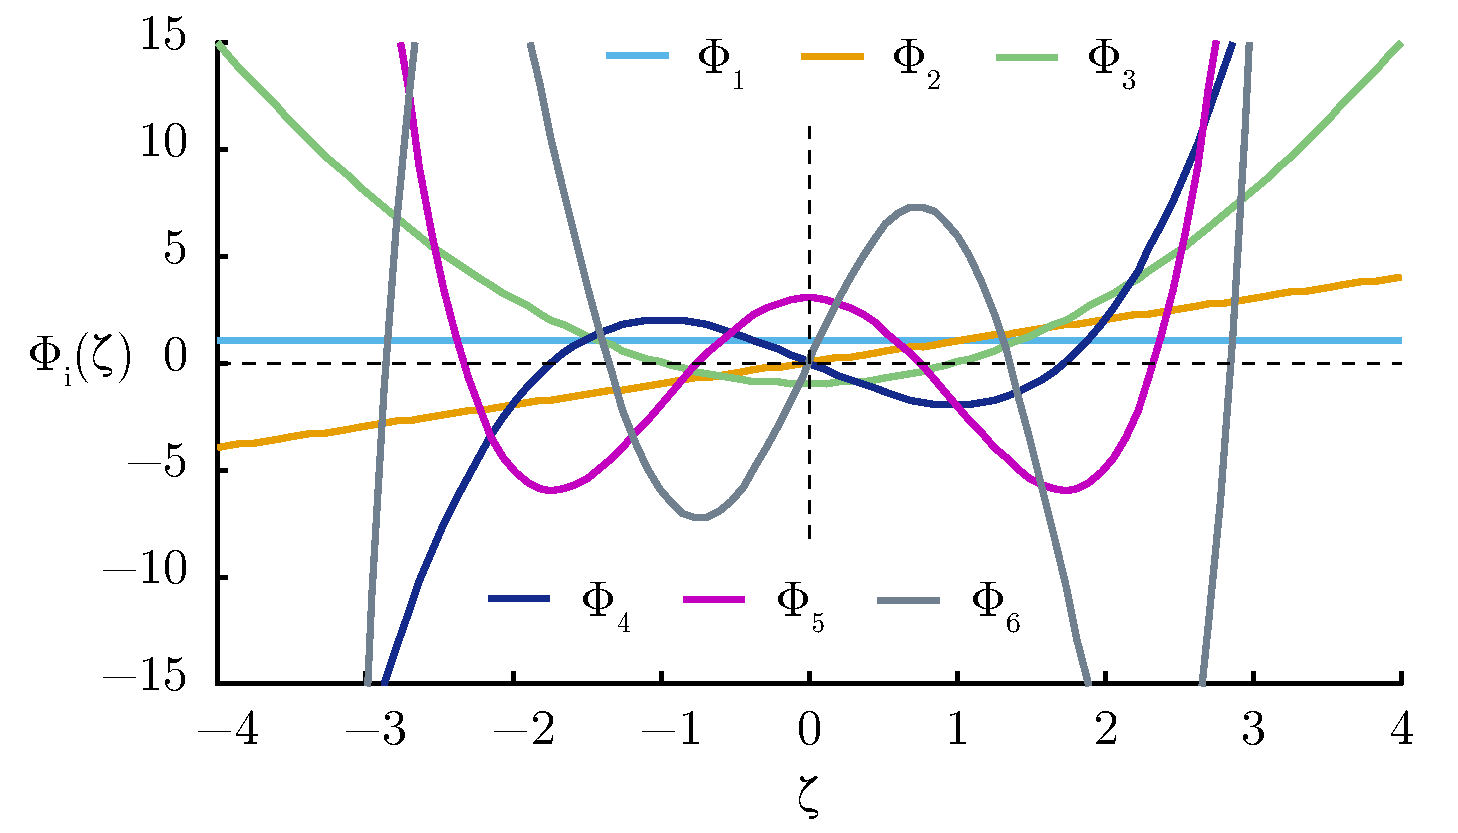
\includegraphics[width=0.9\columnwidth]{include/assets/hermite.pdf}
  }
  \vspace{-1.0em}
  \caption{The first six polynomials of the Hermite basis.}
  \vspace{-1.5em}
  \flabel{hermite}
\end{figure}

The goal now is to transform the ``problematic'' term in \eref{recurrence}, \ie, the power term defined by \eref{power-model}, in such a way that the recurrence in \eref{recurrence} becomes computationally feasible. Our solution is construction of a surrogate model, or, equally, a meta model, for the power model in \eref{power-model}, which we shall further propagate through \eref{recurrence} to obtain an approximation for temperature. To this end, we employ the generalized polynomial chaos (PC) \cite{xiu2002}, which decomposes stochastic quantities into infinite series of orthogonal polynomials of \rvs. Such a series is especially attractive from the post-processing perspective as it is nothing more than a polynomial, the concept that everybody is familiar with; hence, a PC expansion is easy to interpret and is essentially easy to evaluate. A brief introduction to orthogonal polynomials can be found in the appendix, \aref{orthogonal-polynomials}.

The first step towards a PC expansion is the choice of a suitable polynomial basis $\{ \pcb_i(\vz) \}$, which is typically picked from the Askey scheme of hypergeometric orthogonal polynomials \cite{xiu2002}. An example of such a basis, namely, the one composed of Hermite polynomials, is depicted in \fref{hermite}. The step is crucial as the rate of convergence of future expansions closely depends on it. There are no strict rules that guarantee the optimal choice \cite{maitre2010, knio2006}; however, there are best practices which say that one should be guided by the probability distributions of the \rvs\ that drive the stochastic system. The reason for this is that each polynomial basis is orthogonal with respect to a certain weight function (see \aref{orthogonal-polynomials}), and some of such weight functions directly correspond to certain \pdfs; therefore, when these two functions match each other, it can have a positive effect on convergence, even make it exponential \cite{xiu2002}. \tref{askey} in the appendix displays several examples of such paired probability distributions and polynomial bases. For instance, if the \rvs\ $\vZ(\o)$ follow a beta distribution, then the Jacobi basis is worth being tried first. On the other hand, the basis in \fref{hermite} is preferable for Gaussian \rvs; refer to \cite{xiu2010, xiu2002} for further discussions.

Having an appropriate basis chosen, we apply the PC procedure to power in \eref{recurrence} and truncate the resulting infinite series in order to make it feasible for practical implementations. Such an expansion is formally defined as
\begin{equation} \elabel{pc-expansion}
  \oPC{\vars}{\pcorder}{\vP_k(\o)} = \sum_{i = 1}^{\pcterms} \pcc{\vP}_{ki} \; \pcb_i(\vZ(\o))
\end{equation}
where $\{ \pcb_i(\vZ(\o)) \}_{i = 1}^{\pcterms}$ is the truncated basis with $\pcterms$ polynomials terms of $\vars$ variables, and $\pcc{\vP}_{ki} \in \real^\cores$ are the coefficients of the expansion. The latter are computed using spectral projections as it is explained in the appendix, \aref{spectral-projection}. $\pcorder$ denotes the order of the expansion, which determines the maximal degree of the $\vars$-variate polynomials involved in the expansion; hence, $\pcorder$ also defines accuracy.

It can be seen in \eref{recurrence} that, due to the linearity of the operations involved in the recurrence, $\vX_k(\o)$ retains the same polynomial structure as $\vP_k(\o)$. Therefore, using \eref{pc-expansion}, \eref{recurrence} is rewritten as follows, for $k = 1, \dotsc, \steps$:
\begin{equation} \elabel{expanded-recurrence}
  \oPC{\vars}{\pcorder}{\vX_k(\o)} = \mCF_k \: \oPC{\vars}{\pcorder}{\vX_{k-1}(\o)} + \mCS_k \: \oPC{\vars}{\pcorder}{\vP_k(\o)}.
\end{equation}
Thus, there are two PC expansions for two concurrent stochastic processes with the same basis but different coefficients. As shown in \aref{spectral-projection}, \eref{expanded-recurrence} can be reduced to
\begin{equation} \elabel{pc-recurrence}
  \pcc{\vX}_{ki} = \mCF_k \: \pcc{\vX}_{(k - 1)i} + \mCS_k \: \pcc{\vP}_{ki}
\end{equation}
where $k = 1, \dotsc, \steps$ and $i = 1, \dotsc, \pcterms$. Finally, \eref{fourier-output} and \eref{pc-recurrence} are combined together to compute the coefficients of the PC expansion of the temperature vector $\vTO_k(\o)$.

To summarize, the stochastic recurrence in \eref{recurrence}---wherein, in the presence of correlations, an arbitrary functional $\vP_k(\omega)$ of the uncertain parameters $\vU(\o)$ and random temperature $\vTO_k(\o)$ (recall \sref{power-model}) needs to be evaluated and combined with another random vector, $\vX_k(\omega)$---has been replaced with a purely deterministic recurrence in \eref{pc-recurrence} that involves only linear operations. Moreover, looking further in the past, the performed spectral decompositions have substituted the heavy thermal system in \eref{fourier-system} with a light polynomial surrogate defined by a set of basis functions $\{ \pcb_i(\vz) \}_{i = 1}^{\pcorder}$ and the corresponding sets of coefficients, namely, $\{ \pcc{\vP}_{ki} \}_{i = 1}^{\pcorder}$ for power and $\{ \pcc{\vTO}_{ki} \}_{i = 1}^{\pcorder}$ for temperature, where $k$ traverses all $\steps$ time intervals $\dt_k$ of $\profPdyn$. Consequently, the output of the proposed framework constitutes two stochastic profiles, the power $\profP{\o}$ and temperature $\profT{\o}$ profiles, that are ready to be analyzed from the UQ perspective.
